% (C) Marc Lijour, 2018 
% Licensed under a Creative Commons License BY-SA
% https://creativecommons.org/licenses/by-sa/2.5/ca/
% Technical Workshop at Ryerson University, given Feb 27, 2018
% Introduction to Blockchain/Decentralized Application Development
% A primer on Ethereum, on the ConsenSys stack
% 
\frame{
	\frametitle{Who am I?}
	\framesubtitle{\url{https://www.linkedin.com/in/marclijour/}}
	\begin{columns}
	\column{0.5\textwidth}
		\begin{figure}
		
\includegraphics[width=3cm]{../pics/logos/colliderx_logo}
		\end{figure}
	\column{0.5\textwidth}
		\begin{figure}
		
\includegraphics[width=5.5cm]{../pics/logos/consensys-logo-v-630x581}
		\end{figure}
	\end{columns}
}

\frame{
	\frametitle{Access these slides}
	\center\Huge 
	\url{}
}

% 
% ======================================================================================================
%                                     Introduction to Ethereum
% ======================================================================================================
\section{Introduction to Ethereum}
\frame{
	\frametitle{Ethereum}
	%\framesubtitle{}
	\begin{columns}
	\column{0.5\textwidth}
		Ethereum is a \textbf{decentralized platform that runs smart contracts}: applications that run exactly as programmed without any possibility of downtime, censorship, fraud or third party interference.\\
		--- \url{https://ethereum.org}
	\column{0.5\textwidth}
		\begin{figure}
			
\includegraphics[height=6cm]{../pics/ethereum/471px-Ethereum_logo_2014}
		\end{figure}
	\end{columns}
}

\frame{
	\frametitle{A short history of Ethereum}
	Key Milestones:
	\begin{itemize}
		\item (late 2013) Vitalik Buterin describes Ethereum in a paper
		\pause
		\item (Summer 2014) Ethereum raises more than \$14 million in pre-sale
		\pause
		\item (July 30, 2015) Launch of Frontier, initial (beta) version of Ethereum 
		\pause
		\item (March 14, 2016) Launch of Homestead, first production release
		\pause
		\item (Spring 2016) The DAO
		\pause
		\item (July 2, 2016) ETH -- ETC split
		\pause
		\item (October 16, 2017) Launch of Metropolis (vByzantium) --version 3
		\pause
		\item (2017) ETH goes from ~\$7 to more than \$700 (100x increase)
	\end{itemize}
	\vspace{.5em}
	\emph{Check the \href{https://cdn4.benzinga.com/files/images/2017/July/05/invezz-eth-history-base.jpg}{nice infographic (\cite{ethinfographic})}.}\\
	\vspace{.5em}
	More information:\\
	- a ``prehistory'' of the Ethereum protocol (\cite{vbuterin2017:prehistory}).\\
	- the official \href{https://github.com/ethereum/wiki/wiki/White-Paper}{\emph{Ethereum White Paper}}.
}

\frame{
	\frametitle{Store of value}
	\begin{figure}
	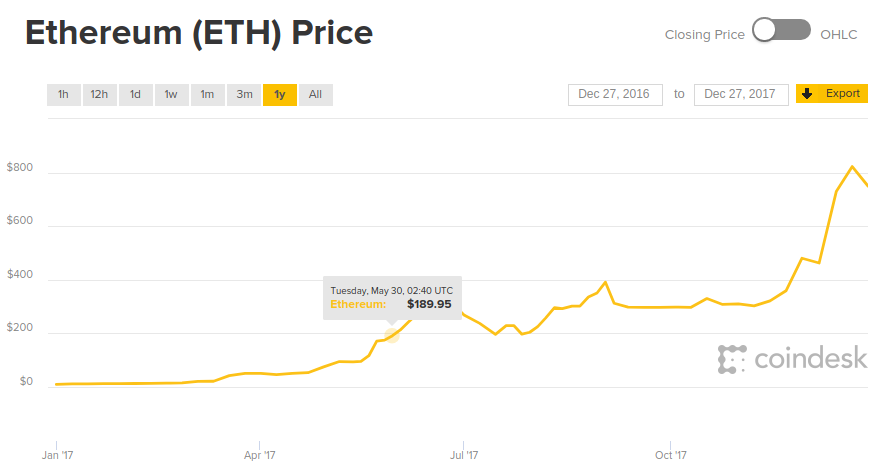
\includegraphics[height=6cm]{../pics/ethereum/ETH-price-2017}
		\caption{ETH price (\cite{coindesk:eth-price})}
		%\caption{Credit: \href{https://www.coindesk.com/ethereum-price/}{Coindesk}}
	\end{figure}
}

\frame{
	\frametitle{Decentralization}
	\begin{figure}
		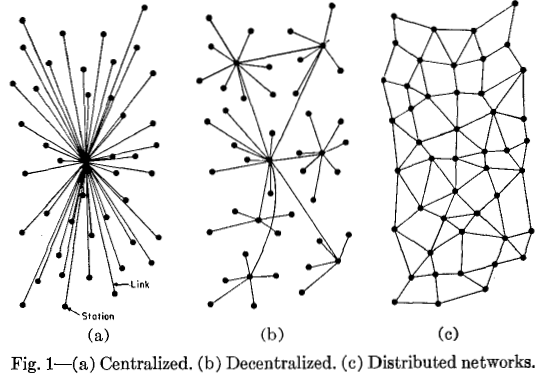
\includegraphics[height=6cm]{../pics/ethereum/networktypes}
	\end{figure}
}

\frame{
	\frametitle{Client Types}
	\begin{itemize}
		\item Full node 
		\pause
		\item Light node 
		\pause
		\item Something in between (e.g. ``fast'' for geth)
	\end{itemize}
}

\frame{
	\frametitle{Disk Space}
	\framesubtitle{Full Archive Ethereum node}
	\begin{figure}
	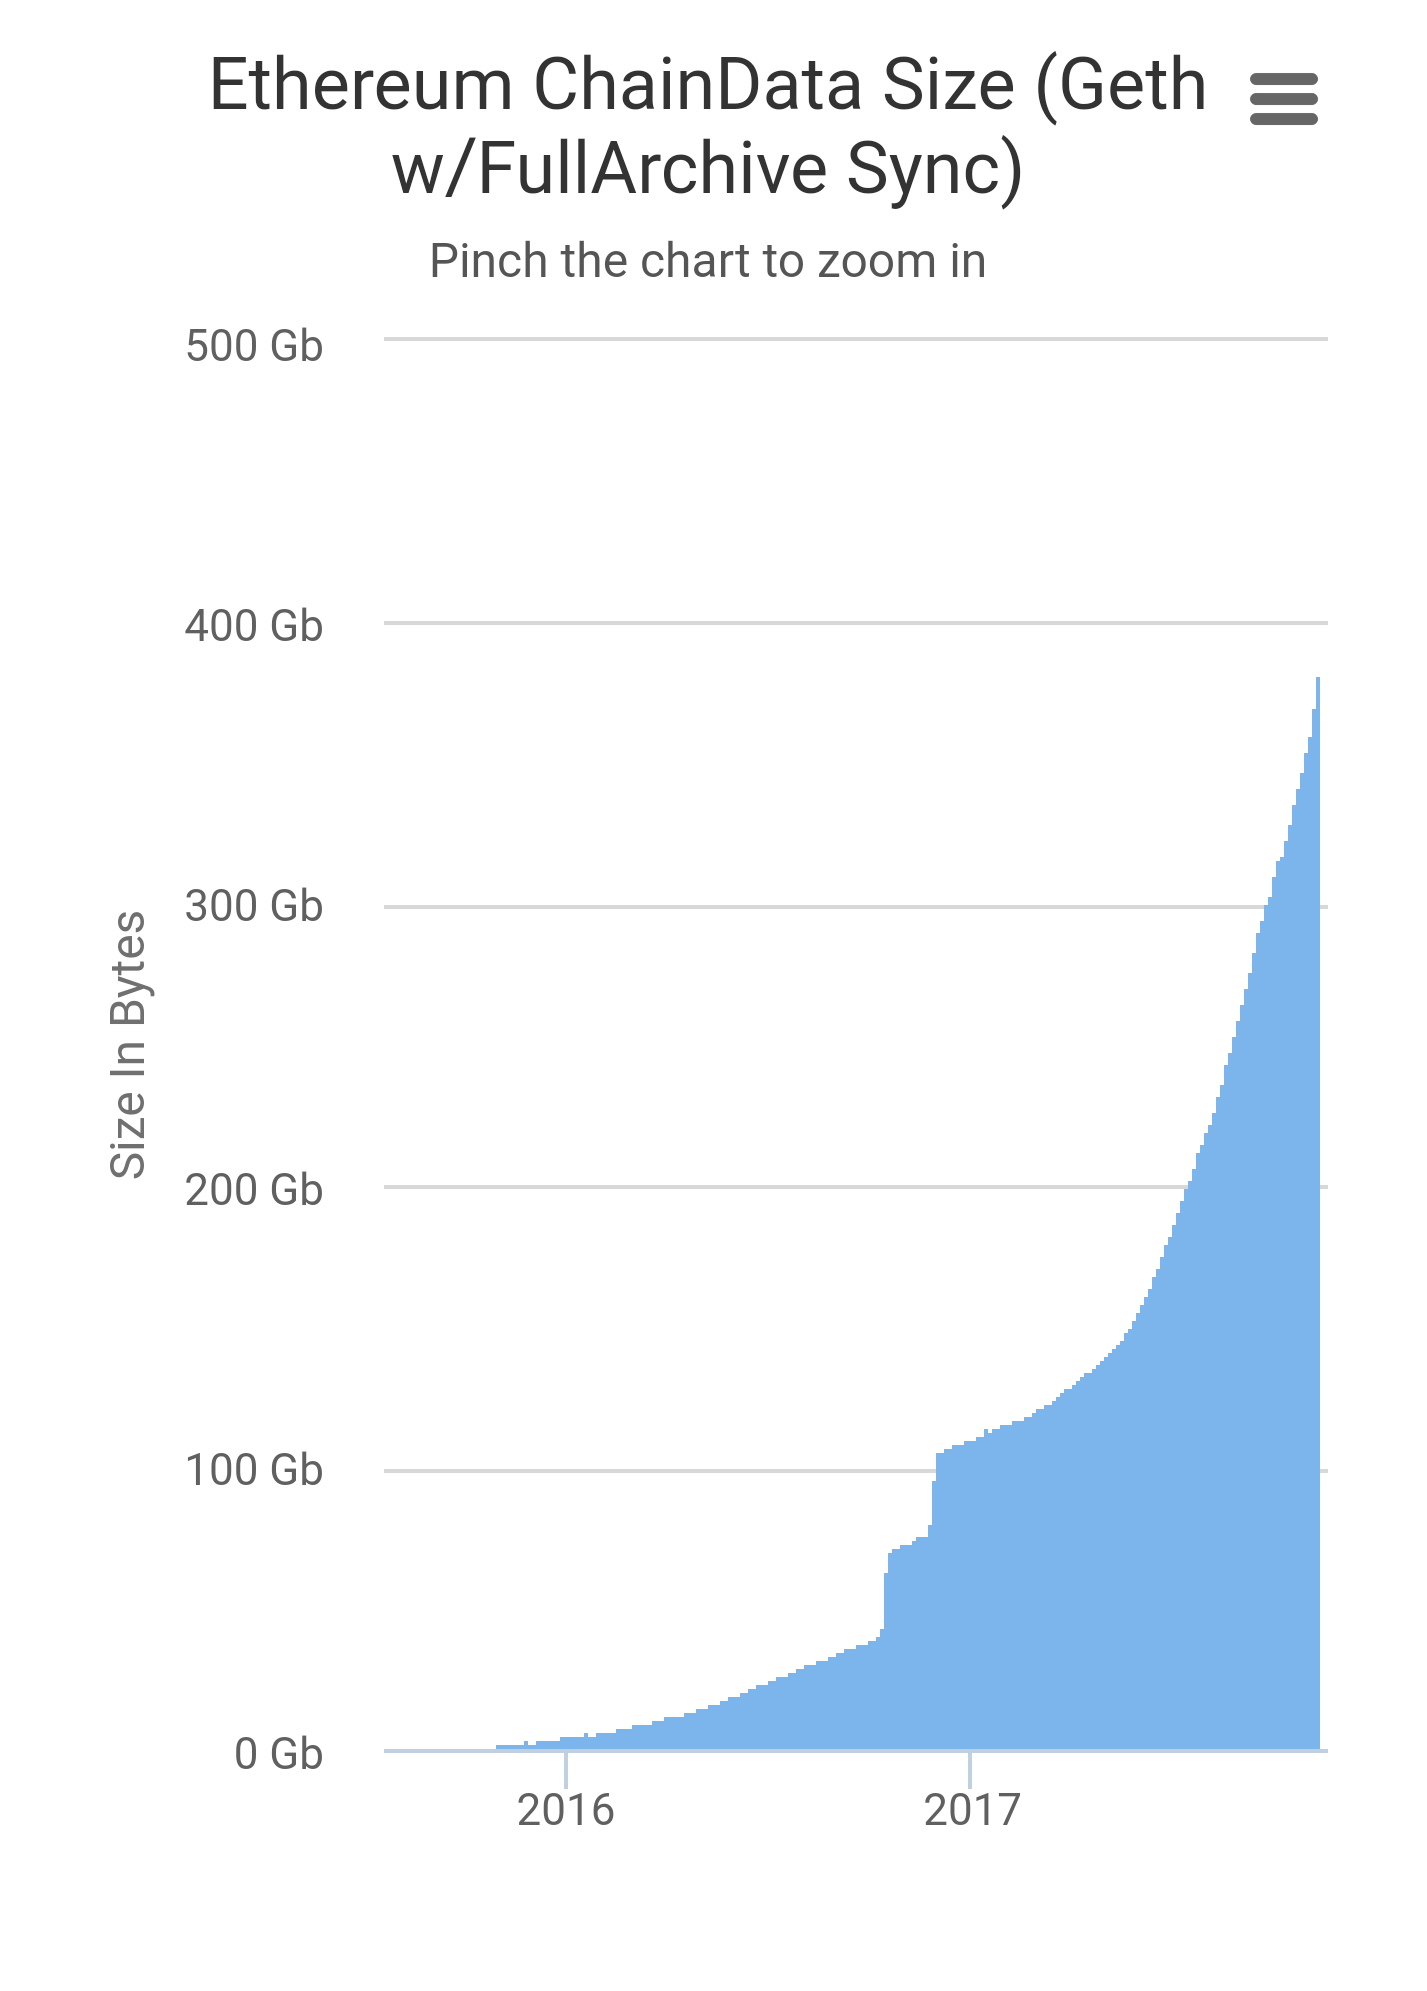
\includegraphics[height=6cm]{../pics/ethereum/geth-full-archive}
		\caption{Miners need a lot of space (\cite{reddit:chaindatasize})}
	\end{figure}
}

\frame{
	\frametitle{Disk Space}
	\framesubtitle{Ethereum vs. Bitcoin}
	\begin{figure}
	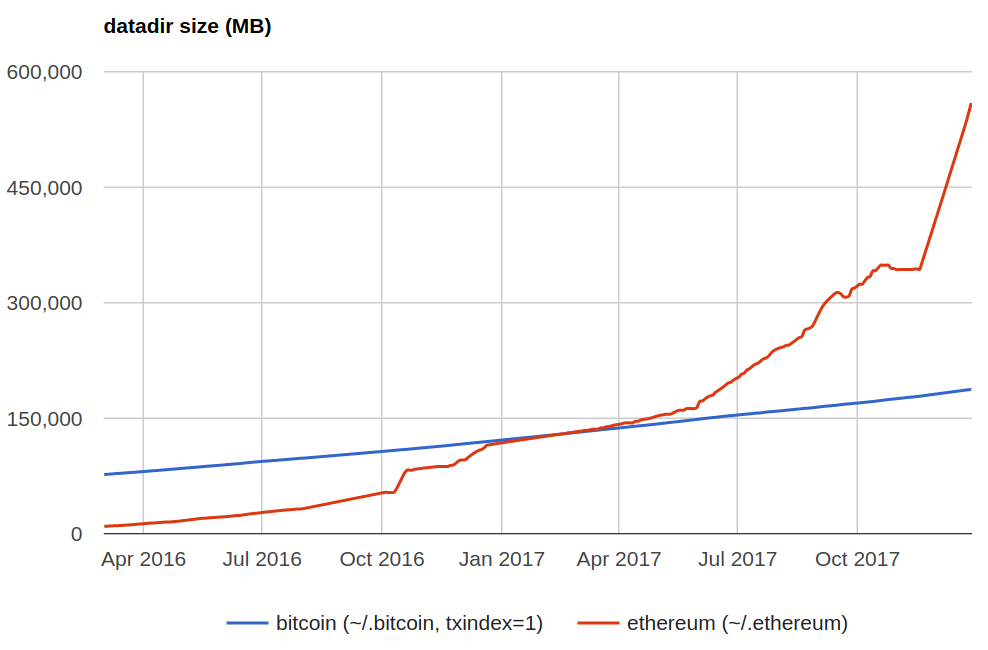
\includegraphics[height=6cm]{../pics/ethereum/daniel_net-datadir_size}
		\caption{Disk space used by Geth (\texttt{fast}) vs. Bitcoin (\cite{daniel:chaindatasize})}
	\end{figure}
}

\frame{
	\frametitle{Disk Space}
	\framesubtitle{With Geth \texttt{--syncmode fast} (default mode)}
	This mode initializes a $\sim$20~GB database, then turns in full node. 
	\begin{figure}
	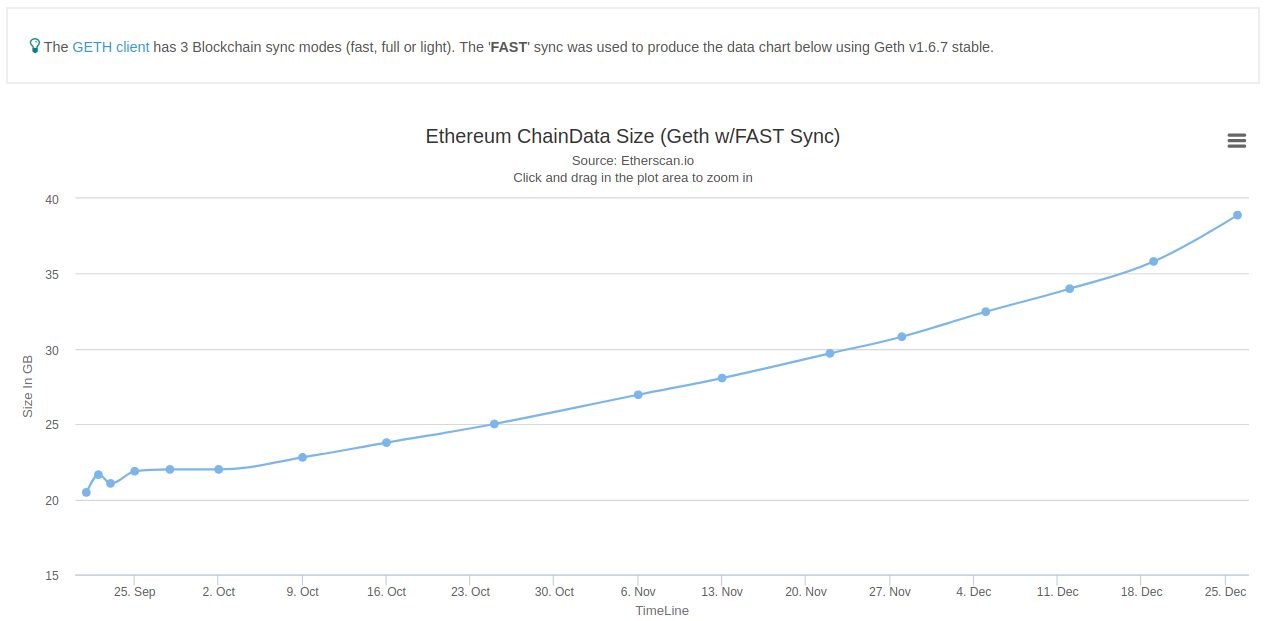
\includegraphics[height=5.5cm]{../pics/ethereum/etherscan-chaindata-2017-12-27}
		\caption{Disk space used by Geth (in fast mode) (\cite{etherscan:chaindatasize})}
	\end{figure}
}

\frame{
	\frametitle{Disk Space}
	\framesubtitle{Parity allows for continuous state trie pruning}
	In green, the configuration running as \emph{full node}.\\
	A light client can fit in $\sim$5~MB.
	\begin{figure}
	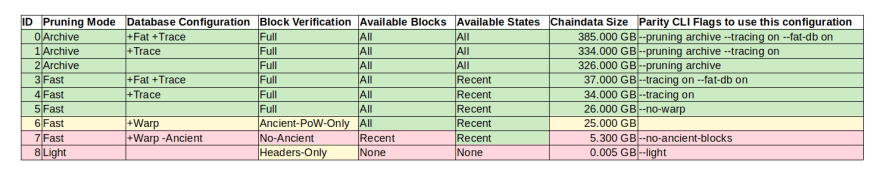
\includegraphics[width=12cm]{../pics/ethereum/afri-parity-size-2017-12}
		\caption{Disk space used by Parity (\cite{afri:chaindatasize})}
	\end{figure}
}

\frame{
	\frametitle{Metamask}
	\begin{figure}
		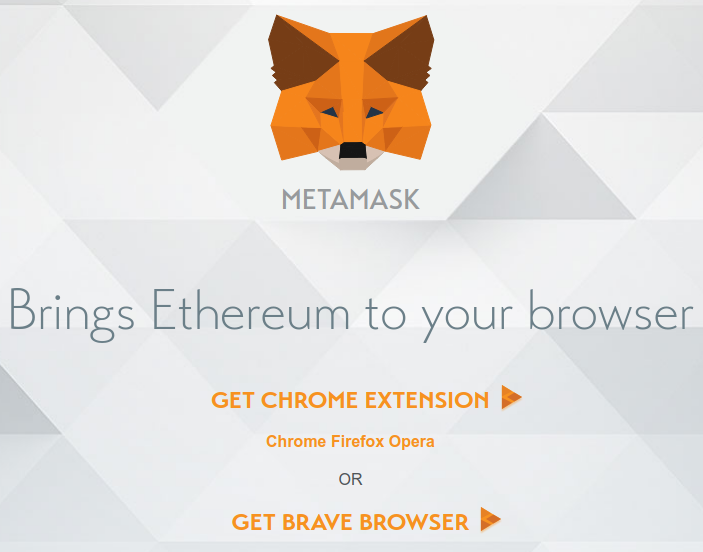
\includegraphics[width=8cm]{../pics/ethereum/metamask-extension}
		\captionsetup{justification=centering}
		\caption*{\url{https://metamask.io}}
	\end{figure}
}

\frame{
	\frametitle{Practical Applications}
	\framesubtitle{for personal or business use}
	\begin{figure}
	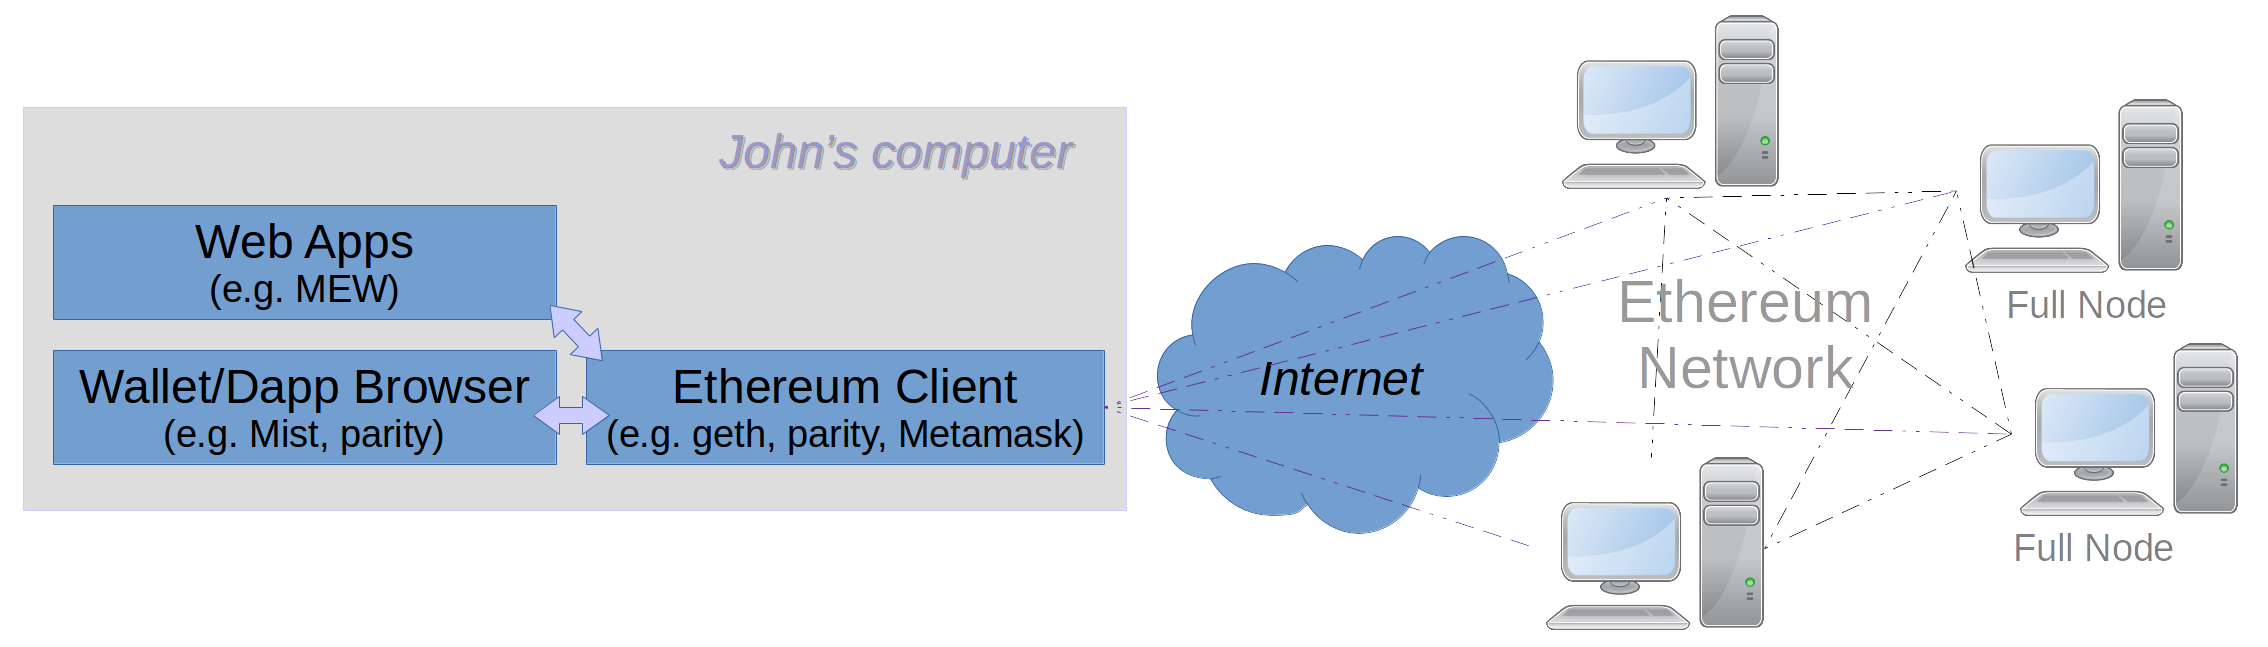
\includegraphics[width=12cm]{../pics/ethereum/ethereum-dapp-arch}
	\end{figure}
}

% ======================================================================================================
%                                     Ethereum dev environment
% ======================================================================================================
\section{Setting a Development Machine}
\frame{
	\frametitle{Sizing up}
	1) Ethereum Node, Wallet, historical data, Smart Contracts, and Dapps:
	\begin{itemize}
		\item Linux machine (Ubuntu 16.04 / Linux Mint 18.x --until April 2021)
		\item Parity (or Geth) 
		\item A Solidity compiler
	\end{itemize}
	\vspace{.7em}
	2) Developer light setup: (works on ChromeOS)
	\begin{itemize}
		\item Chrome browser (or Chromium) --any OS
		\item Metamask Extension
		\item \href{https://remix.ethereum.org}{Remix} IDE
	\end{itemize}
	\vspace{.7em}
	3) Developer Pro setup:
	\begin{itemize}
		\item truffle
	\end{itemize}
}

\frame{
	\frametitle{Parity}
	\begin{figure}
		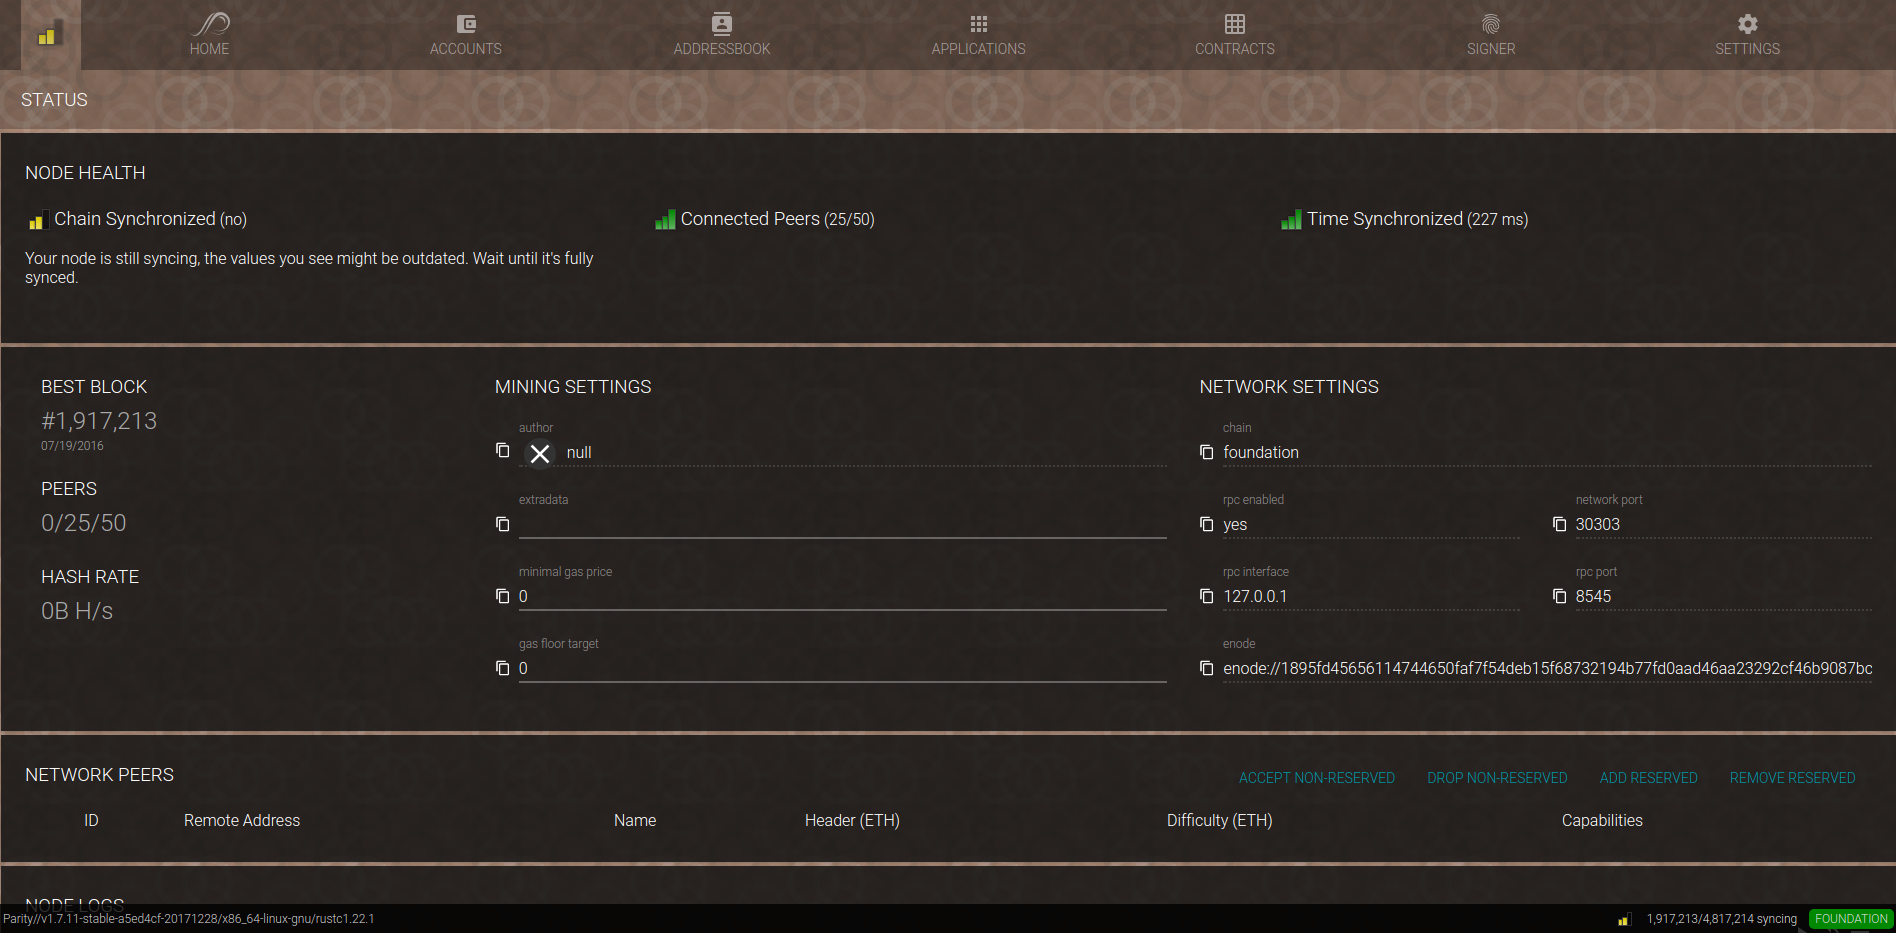
\includegraphics[height=4cm]{../pics/ethereum/parity-status}
		\captionsetup{justification=centering}
		\caption{The \href{https://www.parity.io}{Parity} client syncing}
	\end{figure}
	\vspace{-1em}
	\begin{itemize}
		\item Typical Account Management, multi-sig, hardware support
		\item Access Dapps directly (e.g. app to create an ERC-20 token)
		\item Code editor and Solidity compiler for smart contracts 
		\item Fast and reliable (written in Rust)
		\item Most OS, Docker images; and compliant with JSON-RPC API
	\end{itemize}
}

\frame{
	\frametitle{Lab~1: set up a full Development Environment}
	\center\Huge
	Installing Parity 
}

\frame{
	\frametitle{Installing Parity}
	\begin{figure}
		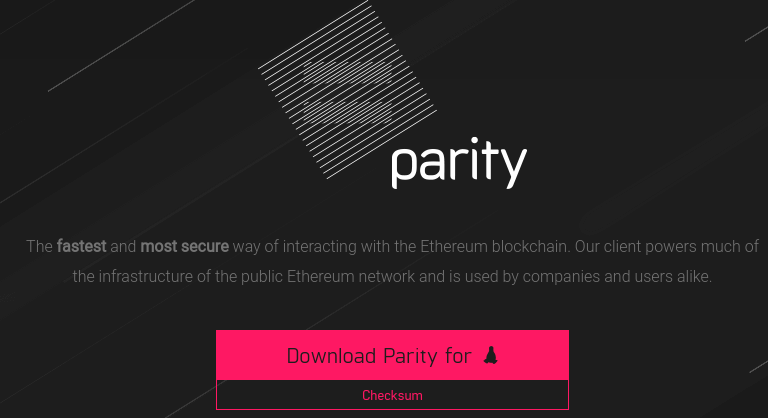
\includegraphics[height=3cm]{../pics/ethereum/parity-homepage}
		\captionsetup{justification=centering}
		\caption*{\tiny\url{https://www.youtube.com/watch?v=WNT2O6xyDmM} (Windows-based, 16~min)}
%		\caption*{\url{https://www.youtube.com/watch?v=sta-p5d1blQ} (older, for Windows)}
	\end{figure}
	\vspace{-1em}
	\begin{enumerate}
		\item Go to \url{https://www.parity.io}
		\item Download the relevant binaries, e.g. on Linux:
		\item Check the checksum: \texttt{\$ md5sum parity\_1.7.11\_amd64.deb}
		\item Install: \texttt{\$ sudo dpkg -i parity\_1.7.11\_amd64.deb}
		\item Check the version: \texttt{\$ parity -v}
	\end{enumerate}
}

\begin{frame}[fragile]
	\frametitle{Run Parity on the Kovan Testnet}
	%\frametitle{Run Parity on the \href{https://github.com/kovan-testnet/config}{Kovan Testnet}}
	\begin{Verbatim}[fontsize=\tiny]
$ parity --light --testnet
2017-12-28 23:38:25  Starting Parity/v1.7.11-stable-a5ed4cf-20171228/x86_64-linux-gnu/rustc1.22.1
2017-12-28 23:38:25  Keys path /home/marc/.local/share/io.parity.ethereum/keys/Kovan
2017-12-28 23:38:25  DB path /home/marc/.local/share/io.parity.ethereum/chains/kovan/db/9bf388941c25ea98
2017-12-28 23:38:25  Path to dapps /home/marc/.local/share/io.parity.ethereum/dapps
2017-12-28 23:38:25  Running in experimental Light Client mode.
...
	\end{Verbatim}
	Then go to \url{http://localhost:8180} (or \url{http://web3.site} if online), and follow the instructions.
	\begin{itemize}
		\item After reading the legal terms and conditions, you can create your first account.
		\item Click on the top left-most logo (yellow bars) to see the status of your node.
		\item \textbf{It may take 60+ minutes to sync!}
	\end{itemize}
\end{frame}

\begin{frame}[fragile]
	\frametitle{Try running your first Dapp}
	Follow the tutorial at \url{https://github.com/paritytech/parity/wiki/Tutorial-Part-1}.\\
	\vspace{1em}
	On Linux Ubuntu, make sure you have npm, and make a soft link to node before running \texttt{init.sh}:
	\begin{Verbatim}[fontsize=\tiny]
$ sudo apt install npm
$ sudo ln -s /usr/bin/nodejs /usr/bin/node 
$ ./init.sh
	\end{Verbatim}	
\end{frame}

\frame{
	\frametitle{Lab~1 (b): set up a full Development Environment}
	\center\Huge
	Installing Geth 
}

\begin{frame}[fragile]
	\frametitle{Installing Geth}
	Instructions (all OS) at \url{https://github.com/ethereum/go-ethereum/wiki/Building-Ethereum}.
	\vspace{.5em}
	\begin{Verbatim}[fontsize=\tiny]
$ sudo apt-get install software-properties-common
$ sudo add-apt-repository -y ppa:ethereum/ethereum
$ sudo apt-get update
	\end{Verbatim}
	Run the first line to install the full suite (geth, bootnode, evm, disasm, rlpdump, ethtest), or the second line for geth only:
	\vspace{.5em}
	\begin{Verbatim}[fontsize=\tiny]
$ sudo apt-get install ethereum
$ sudo apt-get install geth
	\end{Verbatim}
\end{frame}

\begin{frame}[fragile]
	\frametitle{Installing a Solidity Compiler}
	Provided the previous steps were completed:
	\vspace{.5em}
	\begin{Verbatim}[fontsize=\tiny]
$ sudo apt-get install solc
$ which solc
	\end{Verbatim}
And in geth, to let it know where solc can be found:
	\vspace{.5em}
	\begin{Verbatim}[fontsize=\tiny]
$ admin.setSolc("/usr/bin/solc")
	\end{Verbatim}
	Now test the code by following the instructions at \url{https://github.com/ethereum/go-ethereum/wiki/Contract-Tutorial}
\end{frame}

\frame{
	\frametitle{And you still need a wallet}
	\begin{columns}
	\column{0.5\textwidth}
		Options:
		\begin{itemize}
	%		\item Mist = \href{https://www.reddit.com/r/ethereum/comments/61lzmw/mist_ethereum_wallet_myetherwallet/}{Ethereum Wallet (geth) + Web/Dapp browser} --more info \href{https://github.com/ethereum/mist/wiki}{on GitHub}
			\item Mist Browser (beta) (featured on the right, see also the \href{https://blog.ethereum.org/2017/12/15/security-alert-chromium-vulnerability-affecting-mist-browser-beta/}{recent security warning re. Chromium})
			\item \href{https://www.myetherwallet.com}{MyEtherWallet (MEW)} supports advanced features including hardware wallets
		\end{itemize}
	\column{0.5\textwidth}
	\begin{figure}
		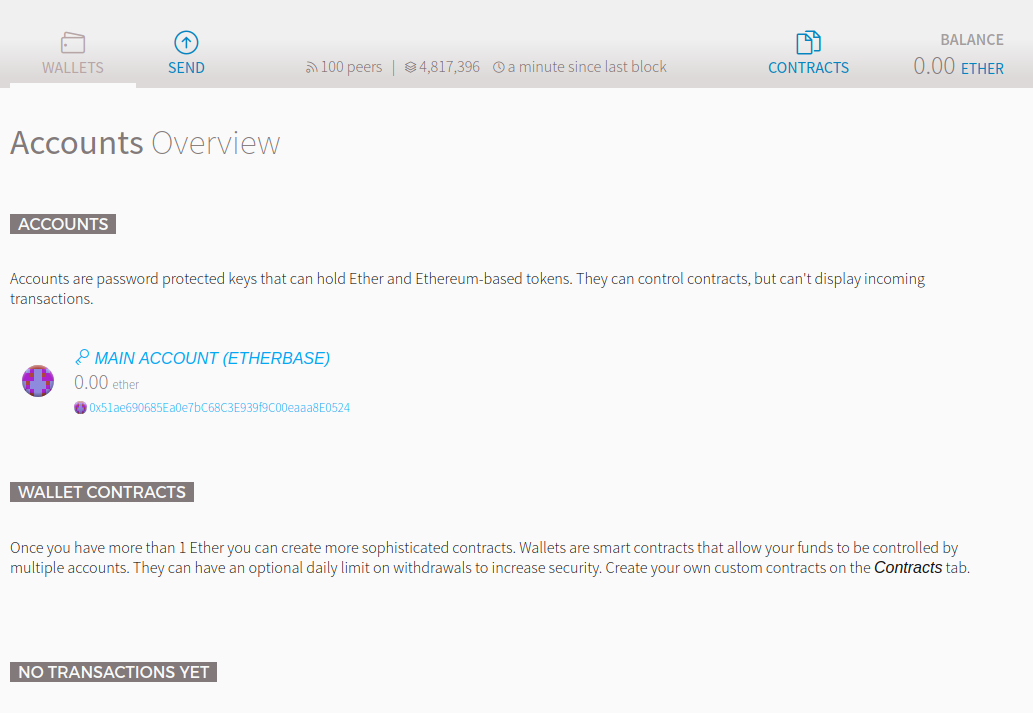
\includegraphics[width=5cm]{../pics/ethereum/mist-browser}
		\captionsetup{justification=centering}
		\caption*{Mist Browser (beta)\newline\url{https://wallet.ethereum.org}}
	\end{figure}
	\end{columns}
}

% ======================================================================================================
%                                     Hands-on Introduction to Smart Contracts 
% ======================================================================================================
\section{Hands-on Smart Contracts}
\frame{
	\frametitle{}
	\centering\Huge
	Let's have some fun!
}

\frame{
	\frametitle{Install MetaMask}
	\begin{columns}
	\column{0.6\textwidth}
		Follow step by step:
		\begin{enumerate}
			\item Install the \href{https://chrome.google.com/webstore/detail/metamask/nkbihfbeogaeaoehlefnkodbefgpgknn}{Chrome/Chromium extension} 
			\item Watch the \href{https://www.youtube.com/watch?v=6Gf\_kRE4MJU}{intro on Youtube}
			\item Create an account 
			\item Switch to the Ropsten Testnet (top-left in MetaMask) 
			\item Fill your account with Ether from \url{https://faucet.metamask.io}
		\end{enumerate}
	\column{0.4\textwidth}
		\begin{figure}
			
\includegraphics[width=3cm]{../pics/ethereum/metamask-logo}
			\captionsetup{justification=centering}
			\caption*{\url{https://metamask.io}}
		\end{figure}
	\end{columns}
}

\frame{
	\frametitle{Create your own (ERC-20) token}
	\begin{figure}
		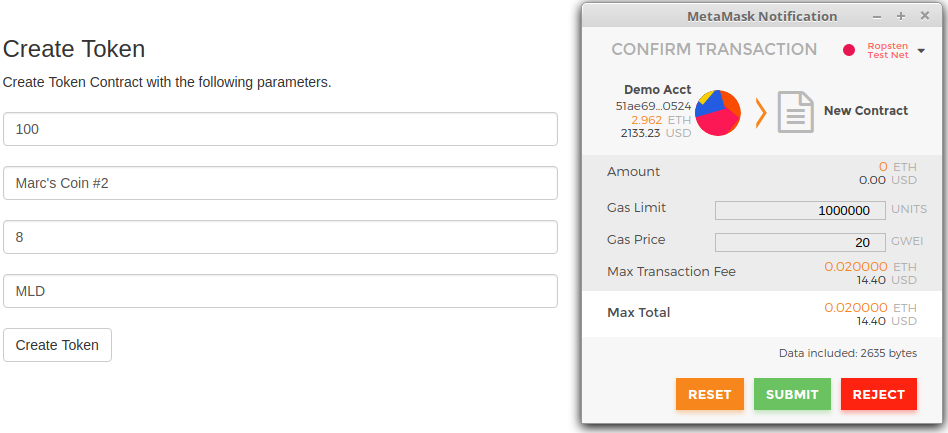
\includegraphics[width=10cm]{../pics/ethereum/token-factory-create}
	\end{figure}
	\vspace{-1em}
	\begin{enumerate}
		\item Use the Token Factory Dapp at \url{https://tokenfactory.surge.sh/\#/factory}
		\item MetaMask will pop up (see picture above)
		\item Submit the transaction (on the Ropsten Testnet)
		\item Check your transaction on \url{https://ropsten.etherscan.io} 
	\end{enumerate}
}

\frame{
	\frametitle{Check your Smart Contract}
	\begin{figure}
		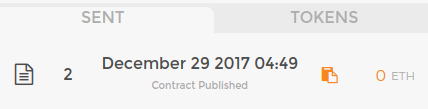
\includegraphics[width=10cm]{../pics/ethereum/metamask-contract-published}
	\end{figure}
	\vspace{-1em}
	\begin{enumerate}
		\item Select the ``Sent'' tab
		\item Check the orange Copy icon (Tx Hash) 
		\item Click on ``Contract Published''
		\item That should bring you to Etherscan (see next page)
	\end{enumerate}
}

\frame{
	\frametitle{Verify the status of your transaction on Etherscan}
	\begin{figure}
		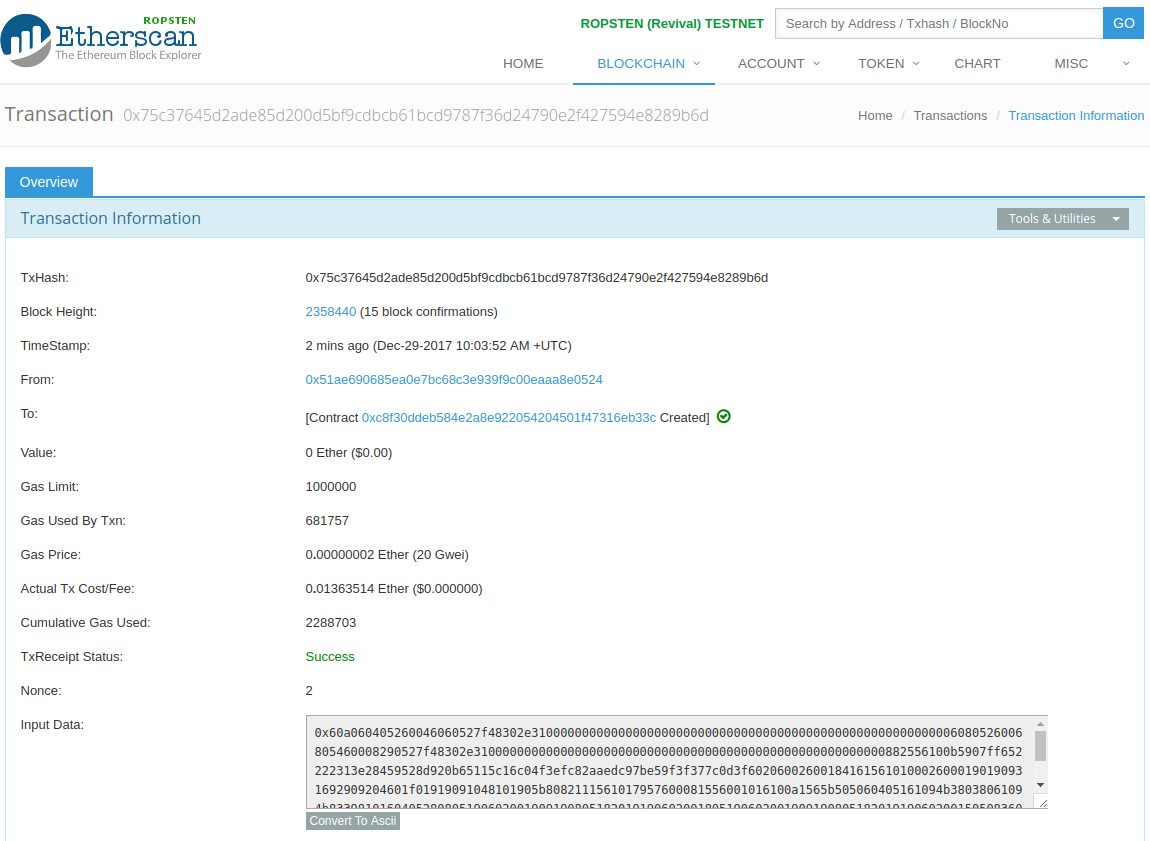
\includegraphics[width=10cm]{../pics/ethereum/etherscan-contract}
		\captionsetup{justification=centering}
		\caption*{Transaction Information: note the ``To'' line with your contract address}
	\end{figure}
}

\frame{
	\frametitle{Watch your Token}
	\begin{columns}
	\column{0.5\textwidth}
		\begin{figure}
			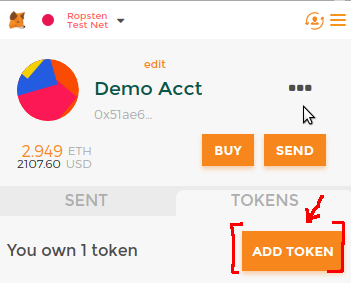
\includegraphics[width=3cm]{../pics/ethereum/metamask-add-token-1}
		\end{figure}
	\column{0.5\textwidth}
		\begin{figure}
			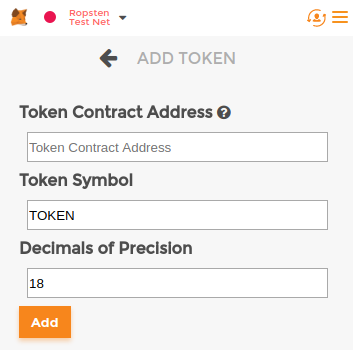
\includegraphics[width=3cm]{../pics/ethereum/metamask-add-token-2}
		\end{figure}
	\end{columns}
	\begin{enumerate}
		\item Click on the ``Add Token'' button
		\item Wait for the next window (picture on the right)
		\item Copy your contract address (from Etherscan)
		\item Go back to your Token Factory tab, which should show an UI to interact with your contract or go to the URL: https://tokenfactory.surge.sh/\#/token/0x... (replace 0x... by your contract address)
		\item Move coins around
		\item In MetaMask, click on your token to check the tx on Etherscan 
	\end{enumerate}
}

\frame{
	\frametitle{}
	\centering\Huge
	Too easy?\\
	\vspace{2em}
	Let's code it in Solidity\\like the pros!
}

\frame{
	\frametitle{Coding your first ERC-20 Smart Contract}
	\begin{figure}
		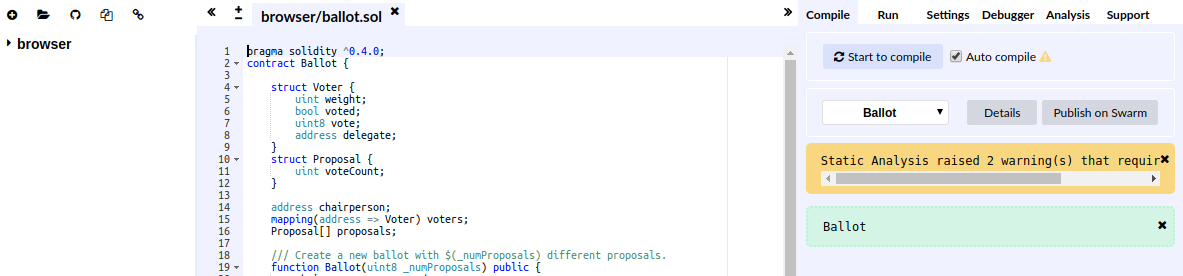
\includegraphics[width=10cm]{../pics/ethereum/remix-home}
	\end{figure}
	\begin{enumerate}
		\item Open the Remix IDE at \url{ https://remix.ethereum.org}
		\item Close the ballot file 
		\item Create a new file named TokenRecipient.sol 
		\item Copy the code from \url{https://ethereum.org/token} (second white box, under ``The Code'', starting with ``pragma'')
		\item Switch to the ``Run'' tab (top-right bar, after Compile)
	\end{enumerate}
	Reference:\\
	\href{https://github.com/ethereum/EIPs/blob/master/EIPS/eip-20-token-standard.md}{ERC-20 Token Standard}
}

\frame{
	\frametitle{Compiling Successfully}
	\begin{figure}
		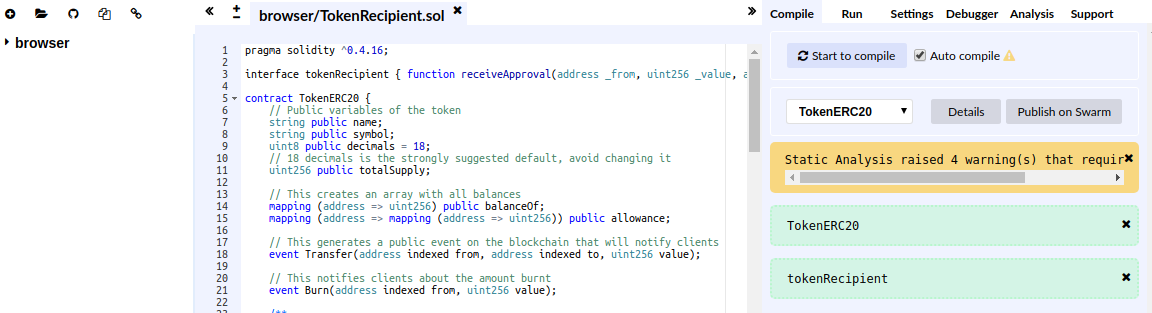
\includegraphics[width=10cm]{../pics/ethereum/remix-compiling-ERC20}
	\end{figure}
	\begin{enumerate}
		\item Two green boxes should show on the right 
		\item TokenERC20 is the name of the contract (class)
		\item tokenRecipient is the name of the interface
		\item Switch to the ``Run'' tab (top right)
	\end{enumerate}
}

\frame{
	\frametitle{Submitting the Smart Contract}
	\begin{figure}
		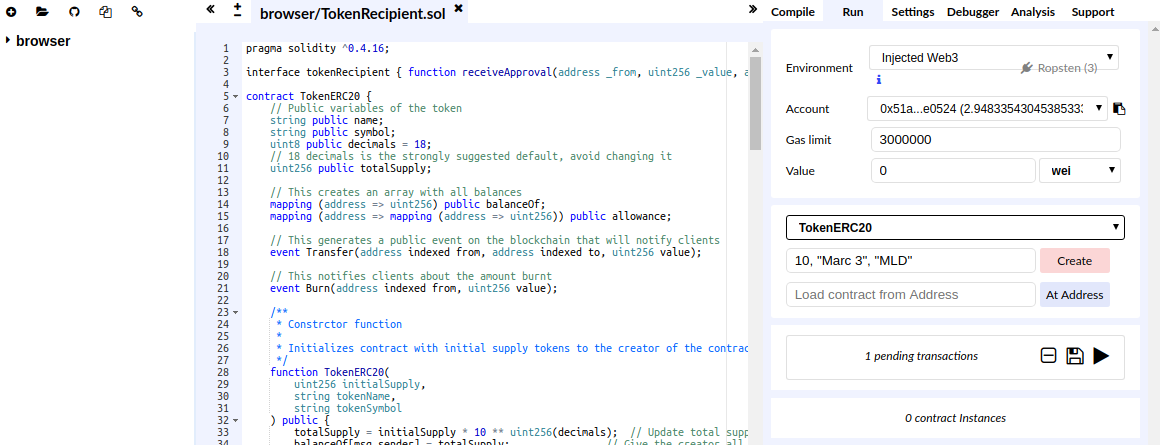
\includegraphics[width=10cm]{../pics/ethereum/remix-creating-ERC20}
	\end{figure}
	\begin{enumerate}
		\item Under the dropdown showing ``TokenERC20'', add a number (total amount of tokens to issue) and two strings (the latter is the token symbol)
		\item Add enough gas (top right, try 30)
		\item Click Create and check whether MetaMask needs confirmation
	\end{enumerate}
}
\frame{
	\frametitle{Interacting with the contract}
	\begin{columns}
	\column{0.4\textwidth}
		\begin{enumerate}
			\item A new interface will pop up on the bottom right corner of the IDE
		\end{enumerate}
	\column{0.6\textwidth}
		\begin{figure}
			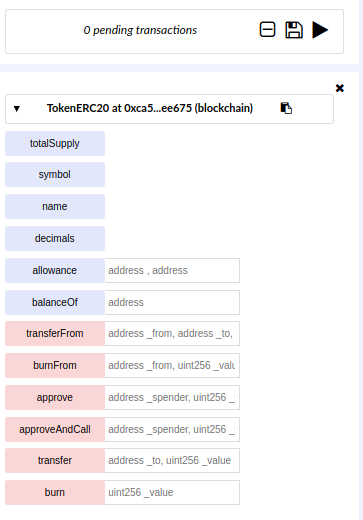
\includegraphics[height=7cm]{../pics/ethereum/remix-ERC20-interact}
		\end{figure}
	\end{columns}
}

\frame{
	\frametitle{}
	\centering\Huge
	Let's create our own permission-based private Blockchain\\
	based on Ethereum!
}

\frame{
	\frametitle{Create a PoA chain with Parity}
	\begin{itemize}
		\item PoA: \href{https://github.com/paritytech/parity/wiki/Proof-of-Authority-Chains}{Proof of Authority}
		\pause
		\item PoA is another type of consensus algorithm (not PoW), with no mining required
		\pause
		\item Less computationally intensive, more secure for small networks, faster
		\pause
		\item The Kovan test network, Hyperledger and Ripple run on a PoA 
		\item Parity supports two PoA consensus algorithm: Aura, and Tendermint (experimental)
		\pause
		\item Let's follow \href{https://github.com/paritytech/parity/wiki/Proof-of-Authority-Chains}{Parity's Demo PoA tutorial}
		\item Simple Hands-on at \url{https://github.com/marclijour/parity-poa-tutorial}
	\end{itemize}
}

\frame{
	\frametitle{Parity's Demo PoA tutorial}
	Objectives:
	\begin{enumerate}
		\item Setup two connected nodes on one machine (for demo)
		\item Gain familiarity with Parity (UI and command line)
		\item Gain a better understanding of diverse types of blockchain (public/private, permissionless/permission-based) and different types of consensus algorithms
	\end{enumerate}
}

\frame{
	\frametitle{Parity's Demo PoA tutorial}
	\framesubtitle{Step 1: download the files}
	This \href{https://github.com/marclijour/parity-poa-tutorial}{tutorial} assumes than you have installed Parity. Instructions are shown for a machine running Linux Ubuntu. The first step consists in cloning the GitHub repo in your machine. You'll run command from within that directory.\\
	\vspace{2em}
	\tiny\texttt{\$ git clone https://github.com/marclijour/parity-poa-tutorial.git}
}

\begin{frame}[fragile]
	\frametitle{Parity's Demo PoA tutorial}
	\framesubtitle{Step 2: create nodes and accounts}
	From the ``parity-poa-tutorial'' directory, open two terminals and type one line in each:
	\vspace{0.5em}
	\begin{Verbatim}[fontsize=\tiny]
$ parity --config node0.starthere
$ parity --config node1.starthere
	\end{Verbatim}
	\vspace{0.5em}
	Open another console and run these scripts:
	\begin{Verbatim}[fontsize=\tiny]
$ ./create_first_authority_address_on_node0.sh
$ ./create_second_authority_address_on_node1.sh
$ ./create_user__address_on_node0.sh 
	\end{Verbatim}
\end{frame}

\begin{frame}[fragile]
	\frametitle{Parity's Demo PoA tutorial}
	\framesubtitle{Step 3: start the chain on PoA}
	In two separate terminals, restart parity with this new configuration.
	\begin{Verbatim}[fontsize=\tiny]
$ parity --config node0.toml
$ parity --config node1.toml
	\end{Verbatim}
\end{frame}

\begin{frame}[fragile]
	\frametitle{Parity's Demo PoA tutorial -- Step 4: setup the Parity UI}
	Open two different windows or tabs in your browser for node 0 (at \url{http://localhost:8181}) and node 1 (at \url{http://localhost:8182}).
	\begin{figure}
		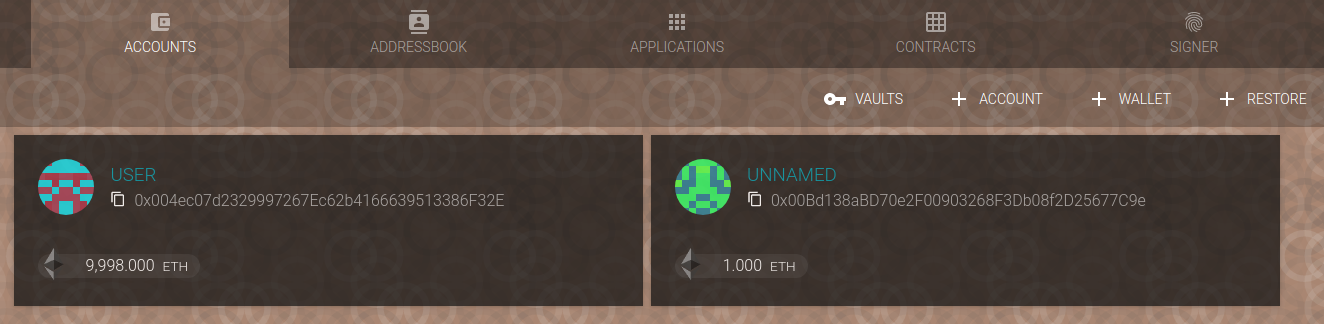
\includegraphics[width=10cm]{../pics/ethereum/parity-poa-tutorial/node0-two-accounts}
	\end{figure}
	Restore the accounts as above:\\
	- on node~0: \texttt{node0} (password = node0), and \texttt{user} (password = user)\\
	- on node~1: \texttt{node1} (password = node1)
\end{frame}

\begin{frame}[fragile]
	\frametitle{Parity's Demo PoA tutorial}
	\framesubtitle{Step 4: connect the nodes with each other}
	Check the console were you started node 0, and look for the Public Node URL. It should ressemble something like this: \texttt{enode://<long hash>@<IP Address>:<Port Number>}
	\begin{figure}
		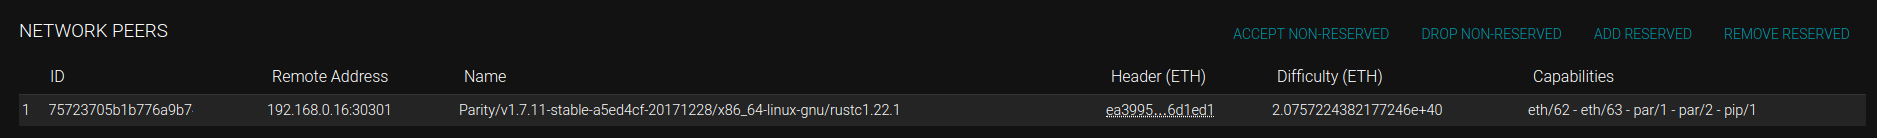
\includegraphics[width=10cm]{../pics/ethereum/parity-poa-tutorial/parity-poa-network-peers}
	\end{figure}
	Go to the Status tab (the leftmost tab) in the Web UI for node 1, and look for the Network Peers section. Click on ADD RESERVED, and copy the URL (including enode://).
	\begin{figure}
		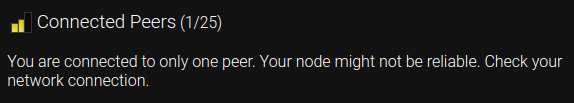
\includegraphics[width=7cm]{../pics/ethereum/parity-poa-tutorial/parity-poa-connected-peers}
	\end{figure}
	Check the console output and the Web UI. Both should acknowledged another peer (1/25 Peers instead of 0/25 Peers).
\end{frame}

\begin{frame}[fragile]
	\frametitle{Parity's Demo PoA tutorial}
	\framesubtitle{Step 5: send transactions}
	Run the following scripts and watch the balance for each account in the Web UIs.
	\begin{Verbatim}[fontsize=\tiny]
$ send_from_user_to_node0_account.sh
$ send_from_user_to_node1_account.sh
	\end{Verbatim}
	You can also try in a separate console, where you can read the JSON-formatted response.
	\begin{Verbatim}[fontsize=\tiny]
$check_balance_in_node0_account.sh
$check_balance_in_node1_account.sh
	\end{Verbatim}
\end{frame}

\begin{frame}[fragile]
	\frametitle{Parity's Demo PoA tutorial}
	\framesubtitle{Step 6: add nodes to the network}
	Run parity with the right chain specification and let other nodes know (by adding them by enode URL). You just need the demo-spec.json file to get started.
	\begin{Verbatim}[fontsize=\tiny]
$ parity --chain demo-spec.json
	\end{Verbatim}
\end{frame}

%\frame{
%	\frametitle{}
%}

\frame{
	\frametitle{}
	\centering\Huge
	It's the beginning of a\\
	rewarding journey...
}

\frame{
	\frametitle{Next Steps and Recommended Readings}
	\begin{itemize}
		\item Starting on Blockchain: \href{https://github.com/marclijour/docs/blob/master/Blockchain/learning.md}{key learning resources}
		\item Fairly exhaustive \href{https://a16z.com/2018/02/10/crypto-readings-resources/}{references from Andreessen Horowitz}
		\item \href{https://github.com/paritytech/parity/wiki}{Parity Wiki} (e.g. \href{https://github.com/paritytech/parity/wiki/Token-Deployment}{Token Deployment})
		\item \href{https://github.com/ethereum/wiki/wiki/White-Paper}{Ethereum White Paper} and \href{https://github.com/ethereum/wiki/wiki}{Wiki}
		\item MOOCs: Udemy (Solidity), edX (Hyperledger)
		\item \href{https://www.amazon.ca/Building-Blockchain-Projects-decentralized-applications-ebook/dp/B01M0DMDDG/ref=sr\_1\_1}{Building Blockchain Projects: Building decentralized Blockchain applications with Ethereum and Solidity} by Narayan Prusty (2017) \emph{--check the section on Proof of Authority (PoA)}
	\end{itemize}
}

